\documentclass[20pt]{extarticle}

% Large-print accommodation copy: bigger base font, single column, tighter
% (but still usable) answer space to avoid excessive page count.
\usepackage[top=0.3in, bottom=0.3in, left=0.35in, right=0.35in]{geometry}
\usepackage{tikz}
\usetikzlibrary{positioning}
\usepackage{enumitem}
\usepackage{graphicx}
\usepackage{tgheros}
\usepackage{ragged2e}
\renewcommand*{\familydefault}{\sfdefault}

\setlength{\parskip}{0pt}

% Ragged-right text avoids overfull lines caused by long inline \texttt{}
% identifiers at this large font size, and is also friendlier to read.
\RaggedRight

% Change this value to resize the grade circle on the quiz header.
\newlength{\gradeCircleRadius}
\setlength{\gradeCircleRadius}{0.45in}

% Set this to the letter identifying this quiz version (e.g. A, B).
\newcommand{\quizVersion}{A}

% Reference diagram of the flash memory map, shown above Question 2 to help
% students locate the bootloader and application regions and their vector
% tables (not to scale).
\newcommand{\flashMapDiagram}{%
\begin{center}
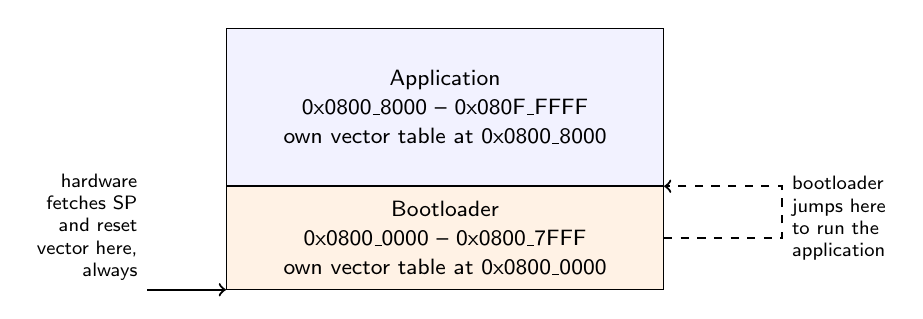
\begin{tikzpicture}[region/.style={draw, align=center, font=\footnotesize, text width=5.2cm, inner sep=5pt}]
\node[region, minimum height=2.0cm, fill=blue!5] (app) {Application\\[1pt] 0x0800\_8000 -- 0x080F\_FFFF\\[1pt] own vector table at 0x0800\_8000};
\node[region, minimum height=1.3cm, fill=orange!10, below=0pt of app] (boot) {Bootloader\\[1pt] 0x0800\_0000 -- 0x0800\_7FFF\\[1pt] own vector table at 0x0800\_0000};
\draw[->, thick] ([xshift=-1.0cm]boot.south west) -- (boot.south west);
\node[anchor=south east, font=\scriptsize, align=right] at ([xshift=-1.0cm]boot.south west) {hardware\\fetches SP\\and reset\\vector here,\\always};
\draw[->, thick, dashed] (boot.east) -- ([xshift=1.5cm]boot.east) |- (app.south east);
\node[right, font=\scriptsize, align=left] at ([xshift=1.5cm,yshift=0.25cm]boot.east) {bootloader\\jumps here\\to run the\\application};
\end{tikzpicture}
\end{center}}

\pagestyle{empty}

\begin{document}

\noindent
\begin{minipage}[t]{\dimexpr\textwidth-2\gradeCircleRadius-0.5in\relax}
    \textbf{ECGR 4101/5101 --- Advanced Embedded Systems}\par
    \textbf{Quiz 2: Startup Process and Bootloaders --- Version \quizVersion\ (Large Print)}\\[6pt]
    Name: \makebox[2.3in]{\hrulefill} \quad Date: \makebox[1.4in]{\hrulefill}
\end{minipage}%
\hfill
\raisebox{0.15in}{%
\begin{minipage}[t]{\dimexpr 2\gradeCircleRadius+0.2in\relax}
    \centering
    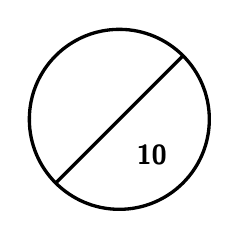
\begin{tikzpicture}[baseline=(circtop.base)]
        \coordinate (circtop) at (0,\gradeCircleRadius);
        \draw[very thick] (0,0) circle (\gradeCircleRadius);
        \draw[very thick] ({\gradeCircleRadius*cos(225)},{\gradeCircleRadius*sin(225)}) -- ({\gradeCircleRadius*cos(45)},{\gradeCircleRadius*sin(45)});
        \node at ({0.36*\gradeCircleRadius},{-0.4*\gradeCircleRadius}) {\textbf{10}};
    \end{tikzpicture}
\end{minipage}}

\vspace{0.05in}
\textit{For each question, circle the letter of the correct answer.}

\vspace{0.05in}

\begin{enumerate}[label=\textbf{\arabic*.}, leftmargin=*, itemsep=2pt]

\item \textbf{(5 points)} There is no operating system on a bare-metal microcontroller to set up memory before your code runs -- the microcontroller's own startup code has to do that job itself.

\begin{enumerate}[label=(\alph*), leftmargin=*, itemsep=6pt]
\item \textbf{(2 points)} Which of the following correctly orders the sequence of events that take place on a generic Cortex-M microcontroller between power-up and the execution of the first instruction in \texttt{main()}?

\begin{center}
\textbf{(A)} SP load $\to$ reset-vector load $\to$ \texttt{main()} $\to$ \texttt{.data} copy $\to$ \texttt{.bss} zero $\to$ early setup

\textbf{(B)} SP load $\to$ reset-vector load $\to$ early setup $\to$ \texttt{.data} copy $\to$ \texttt{.bss} zero $\to$ \texttt{main()}

\textbf{(C)} early setup $\to$ SP load $\to$ reset-vector load $\to$ \texttt{.bss} zero $\to$ \texttt{.data} copy $\to$ \texttt{main()}

\textbf{(D)} SP load $\to$ reset-vector load $\to$ \texttt{.data} copy $\to$ \texttt{.bss} zero $\to$ early setup $\to$ \texttt{main()}
\end{center}
\end{enumerate}

\newpage

\begin{enumerate}[resume, label=(\alph*), leftmargin=*, itemsep=6pt]
\item \textbf{(2 points)} A global variable is declared \texttt{int sensorGain = 5;}. If the startup code's copy of the \texttt{.data} section from flash into SRAM were skipped, what value would \texttt{sensorGain} actually have the first time \texttt{main()} reads it?

\begin{center}
\textbf{(A)} 5 (baked into the machine code)

\textbf{(B)} 0 (SRAM defaults to zero)

\textbf{(C)} Garbage already sitting in SRAM

\textbf{(D)} The program fails to compile
\end{center}

\item \textbf{(1 point)} A global variable is declared \texttt{static int sampleCount;} with no explicit initializer. If the \texttt{.bss} zero-initialization step were skipped at startup, what value would \texttt{sampleCount} have the first time \texttt{main()} reads it?

\begin{center}
\textbf{(A)} 0 (C guarantees it, no hardware needed)

\textbf{(B)} Garbage already sitting in SRAM

\textbf{(C)} 5, same as \texttt{sensorGain}

\textbf{(D)} The program fails to compile
\end{center}
\end{enumerate}

\newpage

\item \textbf{(5 points)} A bootloader and the application it manages are built as two separate programs that share one physical flash chip, as shown below (addresses are representative, not to scale).

\flashMapDiagram

\newpage

\begin{enumerate}[label=(\alph*), leftmargin=*, itemsep=6pt]
\item \textbf{(1 point)} At reset, hardware always fetches the initial stack pointer and reset vector from the same fixed base address of flash (0x0800\_0000). Based on this, which program must be placed at that fixed address?

\begin{center}
\textbf{(A)} The application \quad \textbf{(B)} The bootloader

\textbf{(C)} Either one -- it does not matter \quad \textbf{(D)} A separate ``reset program''
\end{center}

\item \textbf{(2 points)} The bootloader jumps to the application's reset handler without ever changing the processor's vector-table pointer. Immediately afterward, an interrupt fires. Whose interrupt handler actually executes?

\begin{center}
\textbf{(A)} The application's \quad \textbf{(B)} The bootloader's

\textbf{(C)} Neither -- a hard fault, no handler at all \quad \textbf{(D)} Whichever is closest in flash
\end{center}
\end{enumerate}

\newpage

\begin{enumerate}[resume, label=(\alph*), leftmargin=*, itemsep=6pt]
\item \textbf{(1 point)} What is the one action the application's startup code must take so that interrupts are correctly routed to its own handlers instead of the bootloader's?

\begin{center}
\textbf{(A)} Recompile the bootloader without a vector table

\textbf{(B)} Update the vector-table pointer to the application's own table

\textbf{(C)} Move the application's code to 0x0800\_0000

\textbf{(D)} Disable all interrupts permanently
\end{center}

\item \textbf{(1 point)} Why must the bootloader and application be built as two separate projects, each with its own linker script defining a non-overlapping flash region?

\begin{center}
\textbf{(A)} So each can be (re)flashed independently

\textbf{(B)} One linker script cannot produce more than one vector table

\textbf{(C)} They would otherwise be forced to share one stack pointer

\textbf{(D)} It is not required -- only a style preference
\end{center}
\end{enumerate}

\end{enumerate}

\end{document}
